\documentclass[a4paper, 12pt]{article}
\usepackage[margin=2.5cm]{geometry}
\usepackage{amsmath}
\usepackage{graphicx}

\usepackage{setspace}
\onehalfspacing
\setlength{\parindent}{0pt}

\emergencystretch=\maxdimen
\hyphenpenalty=10000

\begin{document}
    Boqian Yu 03708925
	\section{Exercise 3}
        A \texttt{LossFunction} reduces the influence of residual blocks with too large residuals (usually corresponding to outliers), and thus contributes to a more robust Model. E.g. Huber loss:
        \begin{equation*}
        \rho(s)=\left\{\begin{array}{ll}{s} & {s \leq 1} \\ {2 \sqrt{s}-1} & {s>1}\end{array}\right.
        \end{equation*}
        In \texttt{calibration}, all points are guaranteed to be inliers (from \texttt{aprilgrid}), so it is sufficient to only use a \texttt{CostFunction} without filtering the outliers.
        
    \section{Exercise 4}
    \begin{itemize}
        \item Much too large reprojection error: Wrong matches.
        \item Too large reprojection error: Wrong matches.
        \item Too small distance to camera: Wrong matches or wrongly triangulated landmarks stuck in local minima.
        \item Too small z coordinate: Wrong matches or wrongly triangulated landmarks stuck in local minima.
    \end{itemize}
    
    \section{Exercise 5}
        \centering
        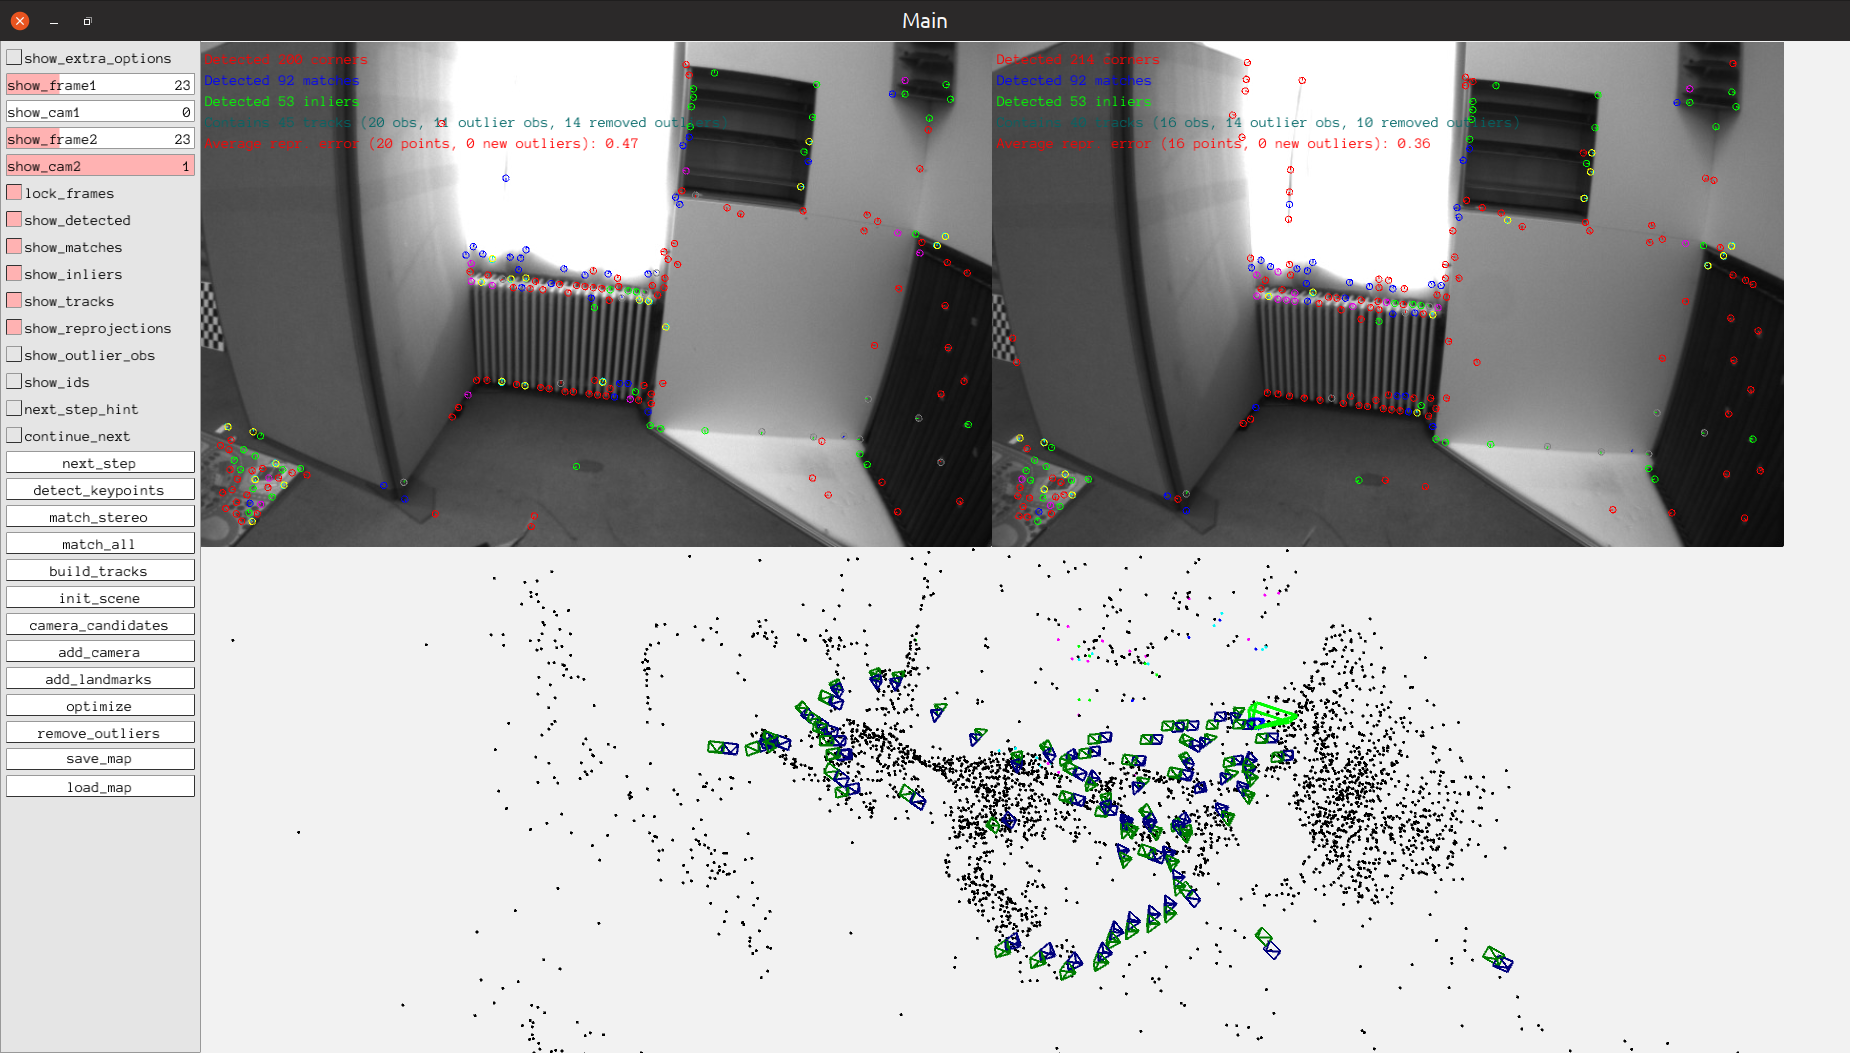
\includegraphics[width=0.9\linewidth]{ex4.png}
        
        \raggedright
        148 cameras are added to the map, taking 116 second. The map-optimization process is taking most of the time, which can possibly be improved by optimizing in each single iteration only parts of the map instead of the whole map, and combining the parts together at last.
\end{document}